%++++++++++++++++++++++++++++++++++++++++
% Don't modify this section unless you know what you're doing!
\documentclass[letterpaper,12pt]{article}
\usepackage{tabularx} % extra features for tabular environment
\usepackage{amsmath}  % improve math presentation
\usepackage{graphicx} % takes care of graphic including machinery
\usepackage[margin=1in,letterpaper]{geometry} % decreases margins
\usepackage{cite} % takes care of citations
\usepackage[final]{hyperref} % adds hyper links inside the generated pdf file
\hypersetup{
        colorlinks=true,       % false: boxed links; true: colored links
        linkcolor=blue,        % color of internal links
        citecolor=blue,        % color of links to bibliography
        filecolor=magenta,     % color of file links
        urlcolor=blue
}
%++++++++++++++++++++++++++++++++++++++++
\usepackage{kotex} % Required for Korean
\usepackage{listings} % for setting code blocks
\usepackage{xcolor} % for using \colorlet
\usepackage{tikz-feynman} % for feynman diagram
\usepackage{amsmath} % for using \usepackage{slashed}
\usepackage{slashed} %for using \slashed

\colorlet{punct}{red!60!black}
\definecolor{background}{HTML}{EEEEEE}
\definecolor{delim}{RGB}{20,105,176}
\colorlet{numb}{magenta!60!black}
\definecolor{dark-green}{rgb}{0.0, 0.5, 0.0}

\begin{document}
\lstdefinelanguage{json}{
    basicstyle=\normalfont\ttfamily,
    numbers=left,
    numberstyle=\scriptsize,
    stepnumber=1,
    numbersep=8pt,
    showstringspaces=false,
    breaklines=true,
    frame=lines,
    backgroundcolor=\color{background},
    literate=
     *{0}{{{\color{numb}0}}}{1}
      {1}{{{\color{numb}1}}}{1}
      {2}{{{\color{numb}2}}}{1}
      {3}{{{\color{numb}3}}}{1}
      {4}{{{\color{numb}4}}}{1}
      {5}{{{\color{numb}5}}}{1}
      {6}{{{\color{numb}6}}}{1}
      {7}{{{\color{numb}7}}}{1}
      {8}{{{\color{numb}8}}}{1}
      {9}{{{\color{numb}9}}}{1}
      {:}{{{\color{punct}{:}}}}{1}
      {,}{{{\color{punct}{,}}}}{1}
      {\{}{{{\color{delim}{\{}}}}{1}
      {\}}{{{\color{delim}{\}}}}}{1}
      {[}{{{\color{delim}{[}}}}{1}
      {]}{{{\color{delim}{]}}}}{1},
}

\title{How to Install \LaTeX{} on WSL}
\author{U. Replica}
\date{\today}
\maketitle

\begin{abstract}
Install \LaTeX{} on WSL and edit it using VS Code.
Then take a look at some examples.
\end{abstract}

\newpage
\section{Install \LaTeX{} Compiler on WSL}
\subsection{Install texlive-full}
\begin{align}
\textbf{\color{dark-green} \underline{sudo} apt \color{black} install texlive-full}
\end{align}

\section{Install LaTeX Workshop Extension in VS Code}
\subsection{Install LaTeX Workshop Extension}
\begin{figure}[ht]
        % read manual to see what [ht] means and for other possible options
        \centering 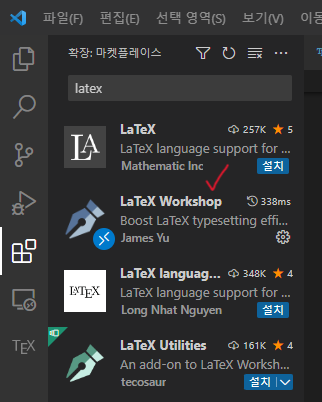
\includegraphics[width=0.4\columnwidth]{latex_workshop.png}
        % note that in above figure file name, "sr_setup",
        % the file extension is missing. LaTeX is smart enough to find
        % apropriate one (i.e. pdf, png, etc.)
        % You can add this extention yourself as it seen below
        % both notations are correct but above has more flexibility
        %\includegraphics[width=1.0\columnwidth]{sr_setup.pdf}
        \caption{
                \label{fig:LaTeX Workshop} % spaces are big no-no withing labels
                % things like fig: are optional in the label but it helps
                % to orient yourself when you have multiple figures,
                % equations and tables
                LaTeX Workshop Extension
        }
\end{figure}

Just install LaTeX Workshop extension. 
It will automatically find the latex compiler.

\subsection{Change LaTeX Workshop Settings}

\begin{lstlisting}[language=json,firstnumber=1,caption={LaTeX Workshop Settings},captionpos=b, label={lst:latex_workshop_settings}]
{"name": "lualatexmk",
	"tools": [
	"lualatexmk"
	]
},
\end{lstlisting}


Go to 파일 > 기본 설정 > 설정 > 확장 > Latex > Latex:Recipes.
Then add the following sentence~\ref{lst:latex_workshop_settings}. 


\section{\LaTeX{} Examples}

\subsection{Equation}

\begin{equation}\label{1.1}
    F = ma
\end{equation}

Force equals mass times acceleration.

\begin{align}
    P &= mv\label{1.2}\\
    E &= mc^2\notag
\end{align}

Momentum equals mass times velocity.
And energy equals mass times the speed of light squared.
As you can see at equation(\ref{1.2}) ~~~

\begin{align}
    e^x &= 1+x+\frac{x^2}{2!}+\frac{x^3}{3!}+\dots\notag\\
    &= \sum^\infty_{n=0} \frac{x^n}{n!}
\end{align}

\begin{equation}
    A = \begin{pmatrix} a & b \\ c & d \end{pmatrix}
\end{equation}

\begin{equation}
        \slashed{p} = \gamma^\mu p_\mu
\end{equation}

\begin{align}
    H = \begin{pmatrix}
    \alpha & 0 & 0 & \\
    0 & \beta & 0 & \ldots \\
    0 & 0 & \gamma & \\
     & \vdots & & \ddots
    \end{pmatrix}\\
    \int^\infty_{-\infty}{\Gamma \alpha e^{\zeta t/\Sigma}dt^4}
\end{align}

\subsection{Table}

\begin{table}[h]
    \centering
    \begin{tabular}{c|cccccc}
    quark & $u$ & $s$ & $t$ & $d$ & $c$ & $b$\\
    \hline
    lepton & $e$ & $\mu$ & $\tau$ & $\nu_e$ & $\nu_\mu$ & $\nu_\tau$
    \end{tabular}
    \caption{This is table}
    \label{table1.1}
\end{table}

\newpage
\subsection{Figure}

\begin{figure}[h]
    \centering
    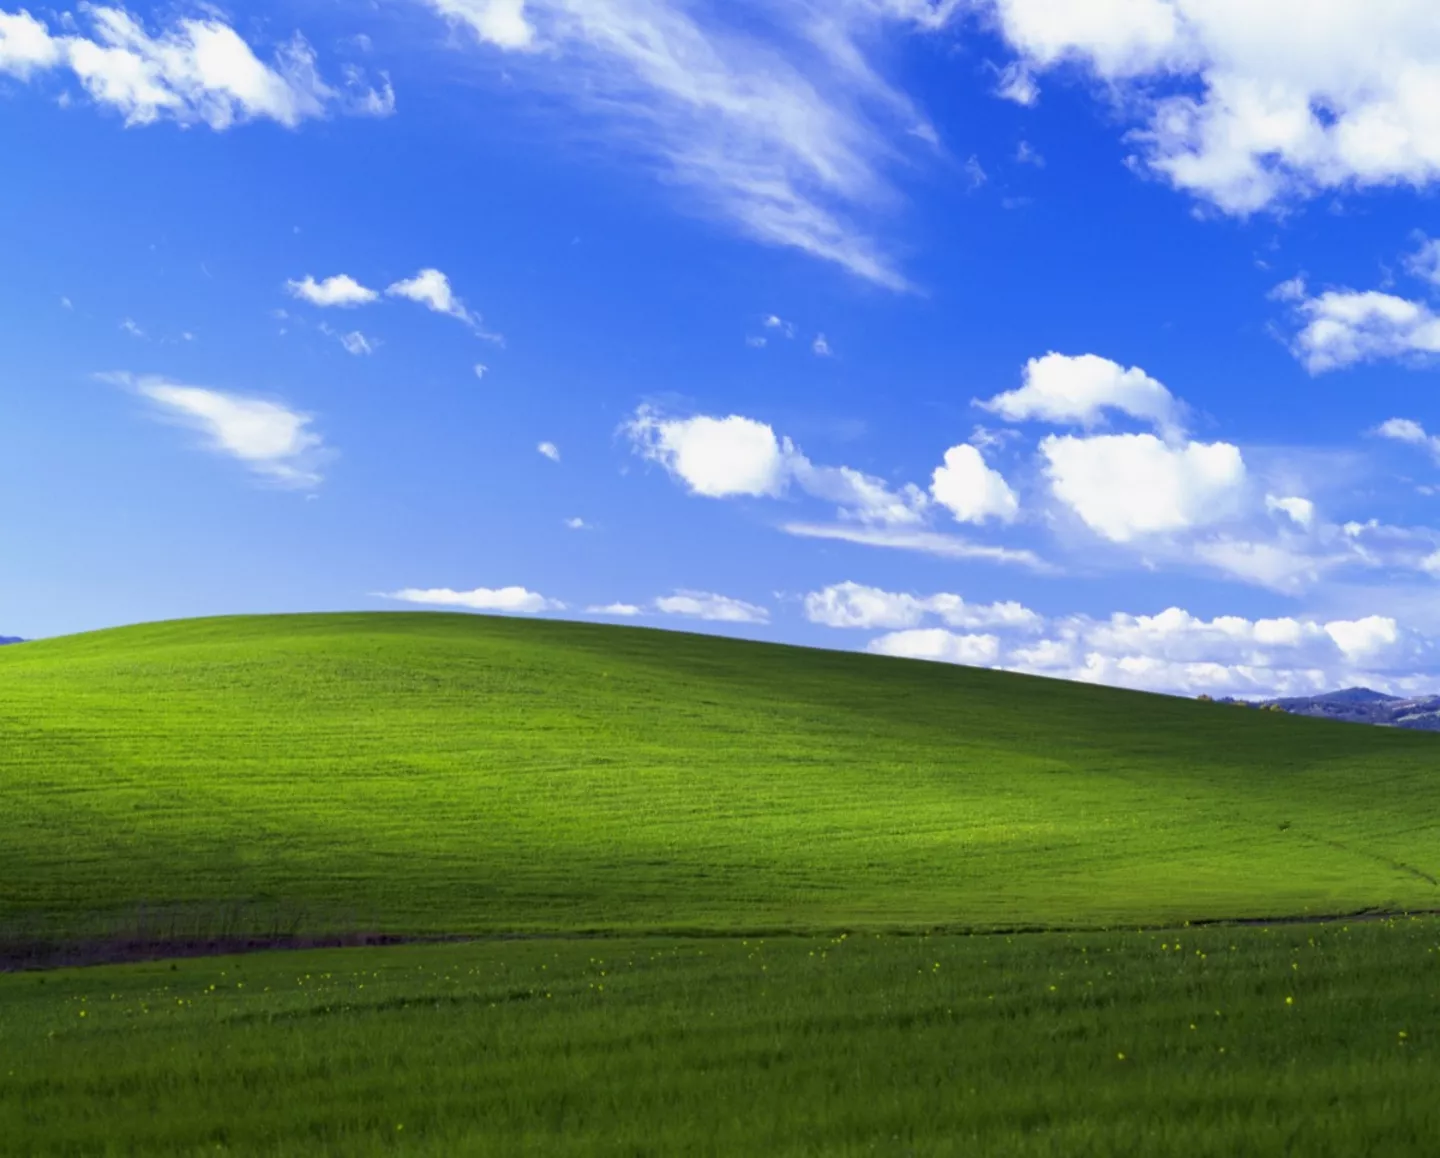
\includegraphics[width=10cm]{wallpaper.png}
    \caption{Wallpaper}
    \label{figure1.1}
\end{figure}

\subsection{Feynman Diagram\cite{TikZ-Feynman}}
\begin{figure}[h]
\centering
\feynmandiagram [horizontal=a to b]{
i1 [particle=\(e^{-}\)] -- [fermion] a -- [fermion] i2 [particle=\(e^{+}\)],
a -- [photon, edge label=\(\gamma\), momentum'=\(k\)] b,
f1 [particle=\(\mu^{+}\)] -- [fermion] b -- [fermion] f2 [particle=\(\mu^{-}\)],
};
\caption{Feynman Diagram}
\label{figure1.2}
\end{figure}
%++++++++++++++++++++++++++++++++++++++++
% References section will be created automatically
% with inclusion of "thebibliography" environment
% as it shown below. See text starting with line
% \begin{thebibliography}{99}
% Note: with this approach it is YOUR responsibility to put them in order
% of appearance.
\begin{thebibliography}{99}

\bibitem{templates} \emph{Sample Lab Report for U of R - PHYS 349}, available at\\
\texttt{https://www.overleaf.com/latex/templates/sample-lab-report-for-u-of-r-phys-349/pgsyqngcyjxk}.

\bibitem{TikZ-Feynman} \emph{TikZ-Feynman Feynman diagrams with TikZ, Version 1.0.0},  available at\\
\texttt{https://arxiv.org/ftp/arxiv/papers/1601/1601.05437.pdf}.

\end{thebibliography}

\end{document}